\chapter{Arhitektura i dizajn sustava}
		\begin{comment}
		\textbf{\textit{dio 1. revizije}}\\

		\textit{ Potrebno je opisati stil arhitekture te identificirati: podsustave, preslikavanje na radnu platformu, spremišta podataka, mrežne protokole, globalni upravljački tok i sklopovsko-programske zahtjeve. Po točkama razraditi i popratiti odgovarajućim skicama:}
	\begin{itemize}
		\item 	\textit{izbor arhitekture temeljem principa oblikovanja pokazanih na predavanjima (objasniti zašto ste baš odabrali takvu arhitekturu)}
		\item 	\textit{organizaciju sustava s najviše razine apstrakcije (npr. klijent-poslužitelj, baza podataka, datotečni sustav, grafičko sučelje)}
		\item 	\textit{organizaciju aplikacije (npr. slojevi frontend i backend, MVC arhitektura) }		
	\end{itemize}
	\end{comment}
	
	Arhitekturu sustava našeg projekta možemo podijeliti na tri glavna podsustava:
	
	\begin{packed_enum}
	
		\item Baza podataka
		\item Web aplikacija
		\item Web poslužitelj
		
	
	\begin{figure}[H]
			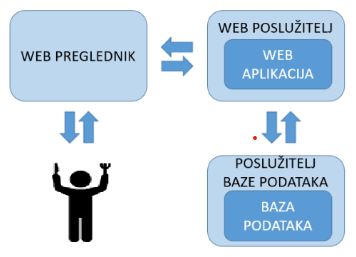
\includegraphics[scale=0.8]{slike/Arhitektura.png} %veličina slike u odnosu na originalnu datoteku i pozicija slike
			\centering
			\caption{Skica arhitekture sustava}
			\label{fig:ARH}
		\end{figure}
		
		
							
	\end{packed_enum}
	
	Internetski preglednik predstavlja programsku platformu koja korisnicima omogućuje pregledavanje web-stranica i konzumiranje raznovrsnih multimedijalnih sadržaja povezanih s njima. Svaki od tih preglednika funkcionira kao svojevrsni tumač, čime interpretira kompleksni kod web stranica i pretvara ga u vizualno prihvatljiv format za korisnike. Bitno je razumjeti da je ključna uloga internetskog preglednika prevesti tehnički zahtjevne  elemente weba u nešto pristupačno svakom korisniku.
	
	Kada korisnik putem internetskog preglednika šalje zahtjev, ta komunikacija se uspostavlja s web poslužiteljem. Web poslužitelj predstavlja temelj rada web aplikacija, a njegova osnovna zadaća je posredovati u komunikaciji između korisnika (klijenta) i same aplikacije. Cijeli taj proces komunikacije odvija se putem HTTP (HyperText Transfer Protocol) protokola, koji služi kao standardni način prijenosa informacija na internetu.

	Važno je naglasiti da je web poslužitelj taj koji pokreće web aplikaciju i prosljeđuje joj korisnički zahtjev. Kroz korištenje web aplikacije, korisnik šalje različite zahtjeve koje aplikacija obrađuje. Ovisno o konkretnom zahtjevu, web aplikacija može pristupiti bazi podataka kako bi došla do relevantnih informacija. Nakon obrade zahtjeva, aplikacija putem web poslužitelja šalje odgovor korisniku u obliku HTML dokumenta. Taj dokument postaje vizualno doživljajan u internetskom pregledniku, predstavljajući krajnji rezultat korisničkog zahtjeva.
	
	Programski jezik kojeg smo odabrali za izradu naše web aplikacije je Java zajedno s React i Spring Boot stackom. Projekt programiramo u razvojnom okruženju Intellj IDEA. Arhitekturu sustava baziramo na MVC konceptu (Model-View-Controller) prilagođenom za React i Spring boot. Glavna karakteristika zbog koje smo se odlučili za MVC je nezavisno razvijanje pojedinih dijelova aplikacije što nam omogućuje jednostavnije testiranje i implementiranje novog koda. Glavna podjela je na tzv. „Backend“ i „Frontend“.
	\vspace{30pt}
	
	
	Backend (Spring Boot) MVC koncept:
	
	\begin{packed_enum}
	
		\item Model: Svi razredi (koje su povezane sa bazom) sa odgovarajućim atributima te servisi u kojima se provodi logika koji kasnije koriste API komponente (Controlleri)
		\item View: JSON podatci s kojima upravljaju API komponente(Controlleri)
		\item Controller: API komponente koje obrađuju zahtjeve te šalju adekvatne odgovore
							
	\end{packed_enum}
	\eject
	
	Frontend (React) MVC arhitektura:
	
	\begin{packed_enum}
	
		\item Model: Stanja i podatci koje se koriste i prikazuju u komponentama
		\item View: Komponente koje reprezentiraju izgled aplikacije odnosno korisničko sučelje
		\item Controller: „Event handleri“ i metode koje obrađuju logiku, unos korisnika te upravljaju podatcima i stanjima u komponentama 
							
	\end{packed_enum}
		

				
		\section{Baza podataka}
			
			Za potrebe našeg sustava koristit ćemo bazu podataka koja svojom strukturom olakšava modeliranje stvarnog svijeta. Osnovna jedinica baze je dokument, definiran svojim imenom i skupom atributa. Dokument može nadovezivati i klasa koja opisuje atribute sadržane u dokumentu. Korištenjem MongoDB-a kao ne-relacijske baze podataka, informacije će biti pohranjene u obliku fleksibilnih dokumenata umjesto tradicionalnih tablica. Zadaća baze podataka je brza i jednostavna pohrana, izmjena i dohvat podataka za daljnju obradu. Baza podataka ove aplikacije sastoji se od sljedećih dokumenata te klasa koje su sadržane unutar njih:
			\begin{packed_item}
	
						\item Korisnik
						
						\item Događanje
							\begin{packed_item}
							\item Mjesto
							\item Foto (lista)
							\item Video (lista)
							\item Recenzije (lista)
							\end{packed_item}
						
						\item Korisnik-Događanje
						
						
						
			\end{packed_item}
			
			Osim dokumenata i klasa u bazi ćemo također imati i vlastite tipove podataka koje će biti prethodno definirani. To su: 
			\begin{packed_item}
	
						\item Uloga
						\item Vrsta
						\item Interes
			\end{packed_item}
						
				
			\subsection{Opis tablica}
			
			\textbf{\large Dokumenti}\\
			

			
			
				%\textit{Svaku tablicu je potrebno opisati po zadanom predlošku. Lijevo se nalazi točno ime varijable u bazi podataka, u sredini se nalazi tip podataka, a desno se nalazi opis varijable. Svjetlozelenom bojom označite primarni ključ. Svjetlo plavom označite strani ključ}
				\textbf{Korisnik} Ovaj dokument sadrži informacije o pojedinačnom korisniku. Sadrži atribute: email, lozinku, ime, prezime, adresu, ulogu, gradove interesa, vrste interesa, web stranicu i facebook. Ovaj dokument je u vezi \textit{One-to-Many} s dokumentom Korisnik-Događanje preko atributa email. Pošto je baza nerelacijska u dokument će se također pisati i liste od: gradova i vrsta koje su potrebne kako bi se izvele sve funkcionalnosti.  
				
				
				
				\begin{longtblr}[
					label=none,
					entry=none
					]{
						width = \textwidth,
						colspec={|X[6,l]|X[10, l]|X[20, l]|}, 
						rowhead = 1,
					} %definicija širine tablice, širine stupaca, poravnanje i broja redaka naslova tablice
					\hline \SetCell[c=3]{c}{\textbf{Korisnik}}	 \\ \hline[3pt]
					\SetCell{LightGreen}Email & STRING	& email korisnika \\ \hline 
					Lozinka	& STRING & hash lozinke\\ \hline 
					Ime	& STRING &   ime korisnika	\\ \hline 
					Prezime & STRING &  prezime korisnika \\ \hline
					Adresa & STRING & kućna adresa korisnika \\ \hline 
					Uloga & ULOGA & uloga korisnika	\\ \hline 
					Gradovi interesa & LIST$<$STRING$>$ & gradovi interesa korisnika \\ \hline 
					Vrste interesa & LIST$<$VRSTA$>$ & vrste interesa korisnika \\ \hline  
					Web stranica & STRING & link web stranice organizatora \\ \hline 
					Facebook & STRING & link facebook profila organizatora \\ \hline
					\end{longtblr}
				
		
			

				\textbf{Događanje} Ovaj dokument sadrži informacije o pojedinačnom događanju. Sadrži atribute: ID, ime, vrsta, mjesto, adresu, datum, vrijeme početka, trajanje, opis, cijenu, foto galeriju, video galeriju i recenzije. Ovaj je dokument u vezi \textit{One-to-Many} s dokumentom Korisnik-Događanje preko atribute ID. Događanje se također nadovezuje na klase mjesto, foto, video i recenziju. Za mjesto bi se moglo reći da je u vezi \textit{One-to-One} jer ima samo jedno mjesto na kojem se događaj može odvijati, a za foto, video i recenzije bi se moglo reći da je u vezi \textit{One-to-Many} jer može imati po više takvih atributa. Zato su ti atributi zapisani u listi.
				
				
				\begin{longtblr}[
					label=none,
					entry=none
					]{
						width = \textwidth,
						colspec={|X[6,l]|X[12, l]|X[20, l]|}, 
						rowhead = 1,
					} %definicija širine tablice, širine stupaca, poravnanje i broja redaka naslova tablice
					\hline \SetCell[c=3]{c}{\textbf{Događanje}}	 \\ \hline[3pt]
					\SetCell{LightGreen}ID & LONG &  	jedinstveni identifikator događanja\\ \hline
					Ime	& STRING &   ime događanja	\\ \hline 
					Vrsta & VRSTA &  vrsta događanja \\ \hline 
					Mjesto & MJESTO	&  grad događanja	\\ \hline 
					Adresa & STRING	& adresa događanja \\ \hline 
					Datum & DATE & datum održavanja	\\ \hline 
					Vrijeme početka & LOCALTIME & vrijeme početka održavanja \\ \hline 
					Trajanje & LOCALTIME & trajanje događanja \\ \hline 
					Opis & STRING & opis događanja \\ \hline 
					Cijena & DOUBLE	&  cijena ulaznice	\\ \hline 
					\SetCell{LightPink}Foto galerija & LIST$<$FOTO$>$ & fotografije događanja \\ \hline 
					\SetCell{LightPink}Video galerija & LIST$<$VIDEO$>$ & videozapisi događanja \\ \hline
					\SetCell{LightPink}Recenzije & LIST$<$RECENZIJA$>$ & recenzije događanja \\ \hline
					\end{longtblr}
				

				\textbf{Korisnik-Događanje}	Ovaj dokument sadrži informacije o odnosu korisnika i događanja. Glavna zadaća mu je da čuva informaciju o tome koji se korisnik izjasni da će doći na koje događanje. Sadrži atribute: email, ID i interes. Sa korisnikom i sa događanjem je povezan \textit{Many-to-One} vezom preko emaila i IDa.
				
				
				\begin{longtblr}[
					label=none,
					entry=none
					]{
						width = \textwidth,
						colspec={|X[6,l]|X[6, l]|X[20, l]|}, 
						rowhead = 1,
					} %definicija širine tablice, širine stupaca, poravnanje i broja redaka naslova tablice
					\hline \SetCell[c=3]{c}{\textbf{Korisnik-Događanje}}	 \\ \hline[3pt]
					\SetCell{LightBlue}Email & STRING & email posjetitelja \\ \hline
					\SetCell{LightBlue}ID & LONG & identifikator događanja \\ \hline
					Interes & INTEREST & interes posjetitelja \\ \hline 
				\end{longtblr}
				
				\eject				
				
				
				
				
				
				\textbf{\large Klase}\\
				
				
				
				\textbf{Mjesto} Ova klasa sadrži informacije o mjestima na kojima se mogu održavati događanja. Atributi mjesta su: ID, ime, poštanski broj, grad i županija. Mjesto je klasa koju koristi događanje u \textit{"relaciji"} \textit{One-to-One}. 
				
				\begin{longtblr}[
					label=none,
					entry=none
					]{
						width = \textwidth,
						colspec={|X[6,l]|X[6, l]|X[20, l]|}, 
						rowhead = 1,
					} %definicija širine tablice, širine stupaca, poravnanje i broja redaka naslova tablice
					\hline \SetCell[c=3]{c}{\textbf{Mjesto}}	 \\ \hline[3pt]
					\SetCell{LightGreen}ID & LONG	&  	jedinstveni identifikator mjesta	\\ \hline
					Ime & STRING & ime mjesta \\ \hline 
					Poštanski broj & INTEGER & datum ostavljanje recenzije  \\ \hline 
					Grad & STRING & grad u kojem se nalazi mjesto  \\ \hline 
					Županija & STRING & županija u kojoj se mjesto nalazi  \\ \hline 
					
				\end{longtblr}
				
				
				
				\textbf{Foto} Ova klasa sadrži informacije o fotografijama koje se nalaze u galeriji događanja. Atributi foto-a su: url i datum. Foto je klasa koja je \textit{"povezana"} s događanjem preko \textit{Many-to-One} veze. 
				
				\begin{longtblr}[
					label=none,
					entry=none
					]{
						width = \textwidth,
						colspec={|X[6,l]|X[6, l]|X[20, l]|}, 
						rowhead = 1,
					} %definicija širine tablice, širine stupaca, poravnanje i broja redaka naslova tablice
					\hline \SetCell[c=3]{c}{\textbf{Foto}}	 \\ \hline[3pt]
					\SetCell{LightGreen}URL & STRING & jedinstveni url fotografije	\\ \hline
					Datum & DATE & datum objave fotografije  \\ \hline 
					
				\end{longtblr}
				
				
				
					
				\textbf{Video} Ova klasa sadrži informacije o videozapisima koji se nalaze u galeriji događanja. Atributi videa su: url i datum. Video je klasa koja je \textit{"povezana"} s događanjem preko \textit{Many-to-One} veze. 
				
				\begin{longtblr}[
					label=none,
					entry=none
					]{
						width = \textwidth,
						colspec={|X[6,l]|X[6, l]|X[20, l]|}, 
						rowhead = 1,
					} %definicija širine tablice, širine stupaca, poravnanje i broja redaka naslova tablice
					\hline \SetCell[c=3]{c}{\textbf{Video}}	 \\ \hline[3pt]
					\SetCell{LightGreen}URL & STRING & jedinstveni url videozapisa \\ \hline
					Datum & DATE & datum objave videozapisa  \\ \hline 
				\end{longtblr}
				
				
				
				
				
				\textbf{Recenzija} Ova klasa sadrži informacije o recenzijama koje su korisnici ostavili na događanja. Ova klasa sadrži atribute: korisničko ime, sadržaj i datum. Recenzija je klasa koja spada pod događanje i s njime je \textit{"povezana"} \textit{Many-to-One} vezom, a s korisnikom je povezana kao u relacijskoj bazi preko emaila \textit{Many-to-One} vezom.
				
				\begin{longtblr}[
					label=none,
					entry=none
					]{
						width = \textwidth,
						colspec={|X[6,l]|X[6, l]|X[20, l]|}, 
						rowhead = 1,
					} %definicija širine tablice, širine stupaca, poravnanje i broja redaka naslova tablice
					\hline \SetCell[c=3]{c}{\textbf{Recenzija}}	 \\ \hline[3pt]
					\SetCell{LightBlue}Email & STRING & email korisnika koji je napisao recenziju  \\ \hline 
					Sadržaj & STRING & sadržaj recenzije \\ \hline 
					Datum & DATE & datum objave recenzije  \\ \hline 
					
				\end{longtblr}
				
				\eject
				
				
				
				
			
			\subsection{Dijagram baze podataka}
				%\textit{ U ovom potpoglavlju potrebno je umetnuti dijagram baze podataka. Primarni i strani ključevi moraju biti označeni, a tablice povezane. Bazu podataka je potrebno normalizirati. Podsjetite se kolegija "Baze podataka".}
				Pošto baza nije relacijska sam dijagram je teže skicirati. Stoga smo radi jednostavnosti odlučili dijagram naše baze skicirati kao da je relacijska. Na dijagramu su dokumenti korišteni u bazi označeni velikim tiskanim slovima, dok su klase koje reprezentiraju atribute u dokumentima označene malim tiskanim slovima i spojene s atributom u kojem se nalaze. U dokumentima su klase pak navedene velikim tiskanim slovima, a one koje se nalaze unutar uglatih zagrada smještene su u listu s više jednakih objekata. Recenzija je jedini rubni slučaj u kojem se korisničko ime zapravo uzima kao foreign key od korisnika, ali je također i u listi atributa u događanju. Program za izradu dijagrama nije imao mogućnost da razdvojimo takve slučajeve pa te veze izgledaju isto.
				
				
		\begin{figure}[H]
			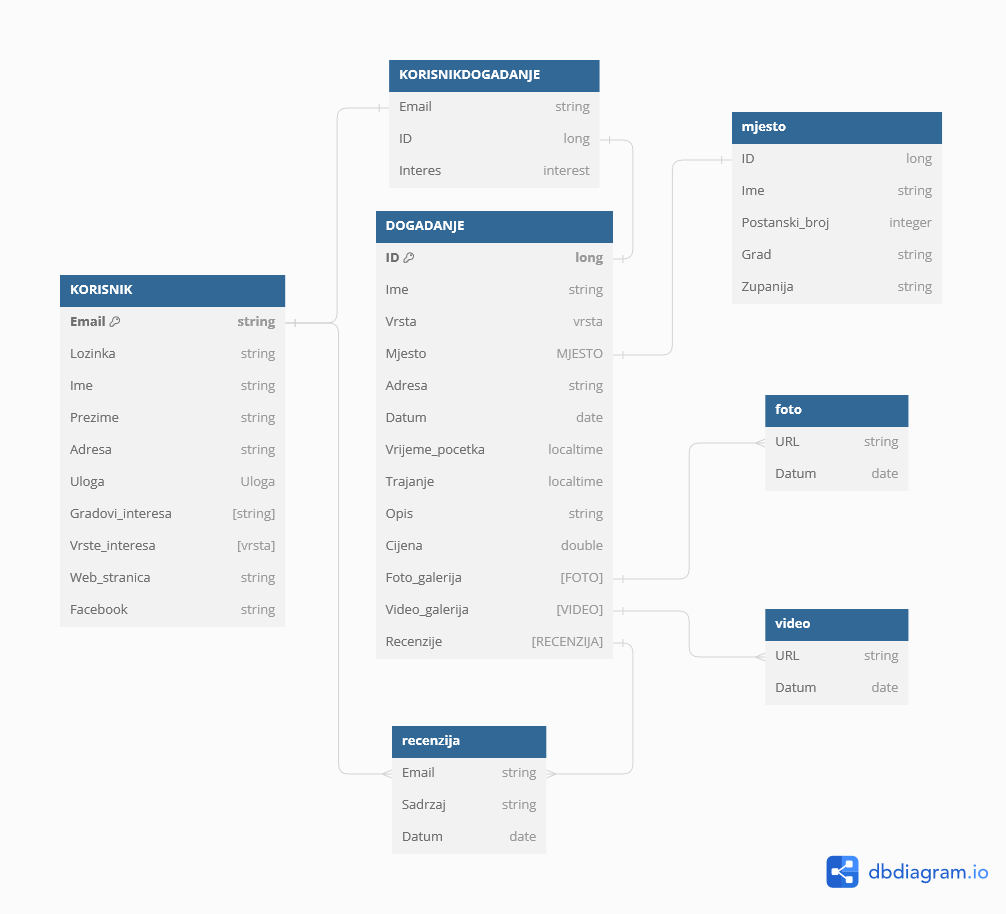
\includegraphics[width=\textwidth]{slike/Dijagram_baza.PNG} %veličina u odnosu na širinu linije
			\caption{Dijagram baze podataka}
			\label{fig:DB} %label mora biti drugaciji za svaku sliku
		\end{figure}
			\eject
			
			
		\section{Dijagram razreda}
		
		
		\begin{comment}
			\textit{Potrebno je priložiti dijagram razreda s pripadajućim opisom. Zbog preglednosti je moguće dijagram razlomiti na više njih, ali moraju biti grupirani prema sličnim razinama apstrakcije i srodnim funkcionalnostima.}\\
			
			\textbf{\textit{dio 1. revizije}}\\
			
			\textit{Prilikom prve predaje projekta, potrebno je priložiti potpuno razrađen dijagram razreda vezan uz \textbf{generičku funkcionalnost} sustava. Ostale funkcionalnosti trebaju biti idejno razrađene u dijagramu sa sljedećim komponentama: nazivi razreda, nazivi metoda i vrste pristupa metodama (npr. javni, zaštićeni), nazivi atributa razreda, veze i odnosi između razreda.}\\
			
			\textbf{\textit{dio 2. revizije}}\\			
			
			\textit{Prilikom druge predaje projekta dijagram razreda i opisi moraju odgovarati stvarnom stanju implementacije}
		\end{comment}
		
			Na slikama \ref{fig:DRC} i \ref{fig:DRM} prikazani su razredi koji pripadaju backend dijelu arhitekture aplikacije. Razredi prikazani na slici \ref{fig:DRC} nasljeđuju razred Controller i primarno služe za dohvaćanje i manipulaciju podataka u sustavu. Na slici \ref{fig:DRM} prikazan je dijagram koji preslikava strukturu baze podataka. Metode u tim razredima direktno komuniciraju s bazom podataka. Razred User predstavlja korisnika čiju vrstu određuje enumeracija Role. Ovisno o vrijednosti te enumeracije, može se raditi o posjetitelju, administratoru ili organizatoru. Razred Event predstavlja objavljeno događanje koje je vrste određene vrijednosti enumeracije EventType. Razred Event kao atribute sadrži listu objekata razreda Photo i listu objekata razreda Video. Dva navedena razreda predstavljaju redom fotografije i videozapise događanja. Razred Event također sadrži listu objekata razreda EventUser. Razred EventUser predstavlja oznaku kojom je korisnik označio određeni događaj. Taj razred dakle povezuje korisnika s nekom vrijednosti iz enumeracije Interest. Razred Event također sadrži listu objekata razreda Review koji predstavlja recenzije koje su korisnici ostavili za određeno događanje.
		
		
		\begin{figure}[H]
			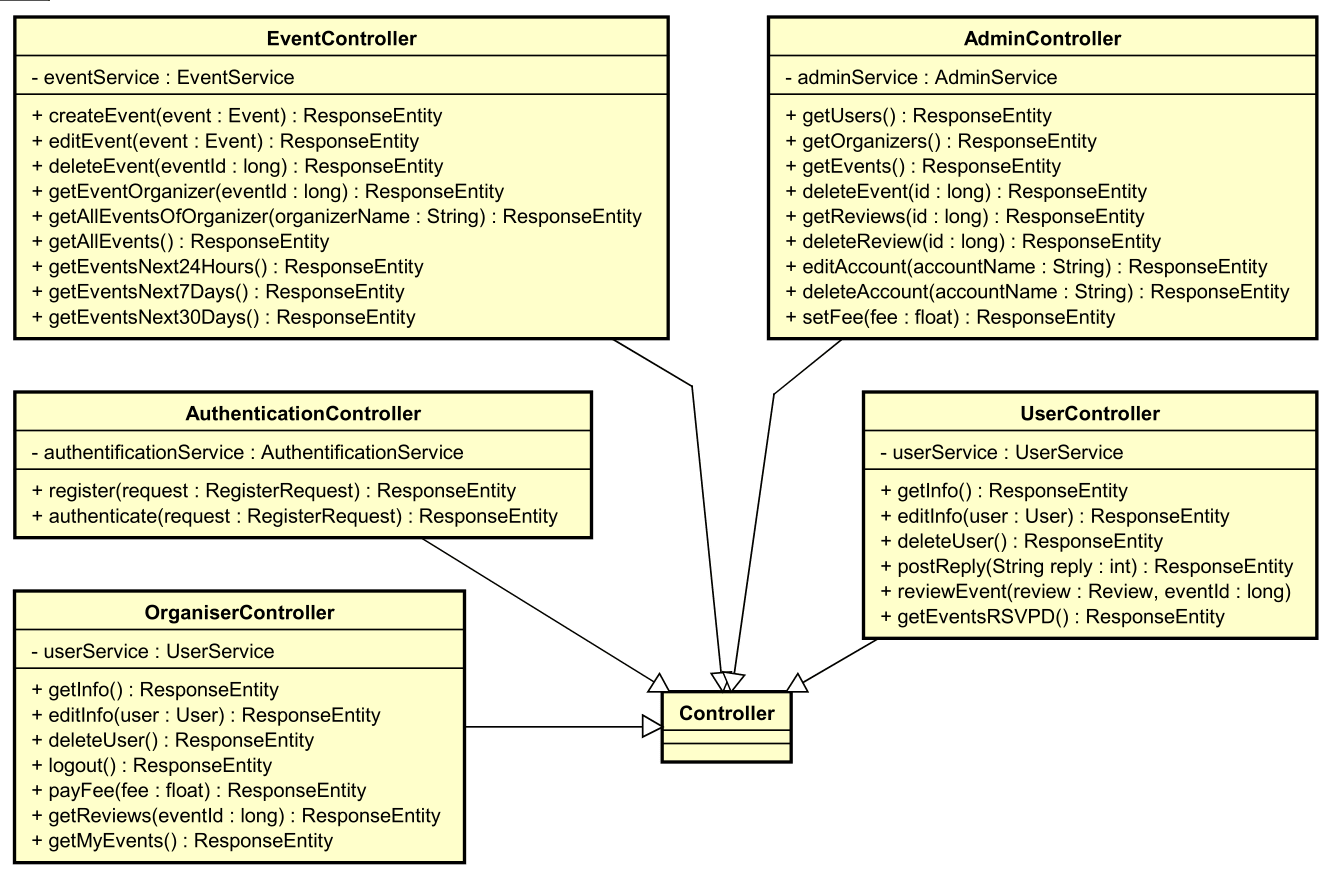
\includegraphics[width=\textwidth]{slike/DRC-1.PNG} %veličina u odnosu na širinu linije
			\caption{Dijagram razreda - Controllers}
			\label{fig:DRC} %label mora biti drugaciji za svaku sliku
		\end{figure}
			
			
		\begin{figure}[H]
			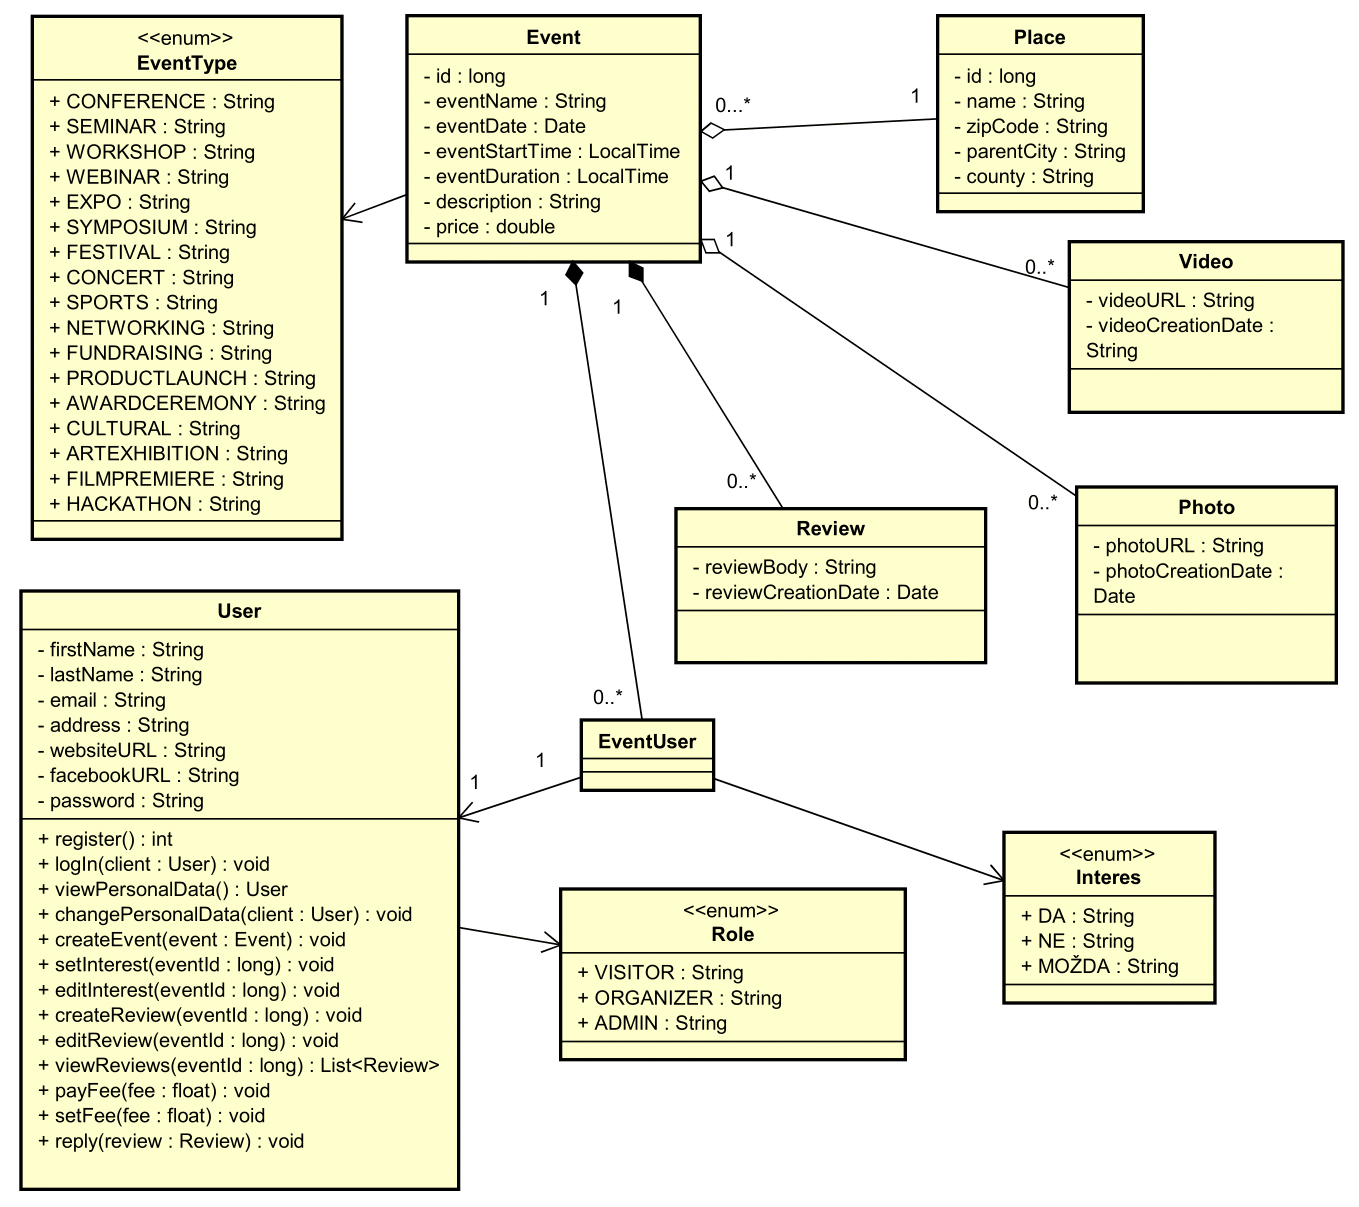
\includegraphics[width=\textwidth]{slike/DRM-1.PNG} %veličina u odnosu na širinu linije
			\caption{Dijagram razreda - Models}
			\label{fig:DRM} %label mora biti drugaciji za svaku sliku
		\end{figure}
			
			
			\eject
		
		\section{Dijagram stanja}
			
			\begin{comment}
			\textbf{\textit{dio 2. revizije}}\\
			
			\textit{Potrebno je priložiti dijagram stanja i opisati ga. Dovoljan je jedan dijagram stanja koji prikazuje \textbf{značajan dio funkcionalnosti} sustava. Na primjer, stanja korisničkog sučelja i tijek korištenja neke ključne funkcionalnosti jesu značajan dio sustava, a registracija i prijava nisu. }
			\end{comment}
			
			Dijagram stanja prikazuje stanja objekta te prijelaze iz jednog stanja u drugo temeljene na dogadajima. Slika \ref{fig:DSP} prikazuje dijagram stanja prijavljenog posjetitelja. Nakon prijave posjetitelju se na početnoj stranici prikazuje lista budućih događanja. Odabere li posjetitelj određeno događanje bit će mu ponuđene opcije da pročita više o događanju, označi dolaznost na događanje te da pogleda profil organizatora. Ako posjetitelj odabere pogledati profil organizatora otvoriti će mu se stranicu u kojoj će moći vidjeti recenzije ostaljene na neka događanja organizatora, buduća i prošla događanja te podatke o samom organizatoru. Ako posjetitelj želi pregledati svoj profil to će moći napraviti tako da odabere "Profil". Na toj će stranici moći pogledati i urediti svoje podatke, obrisati svoj račun, promjeniti interes za svoja buduća događanja, ostaviti osvrt na događanje na kojem je bio te urediti ili obrisati recenziju koju je već napisao.
			
			\begin{figure}[H]
			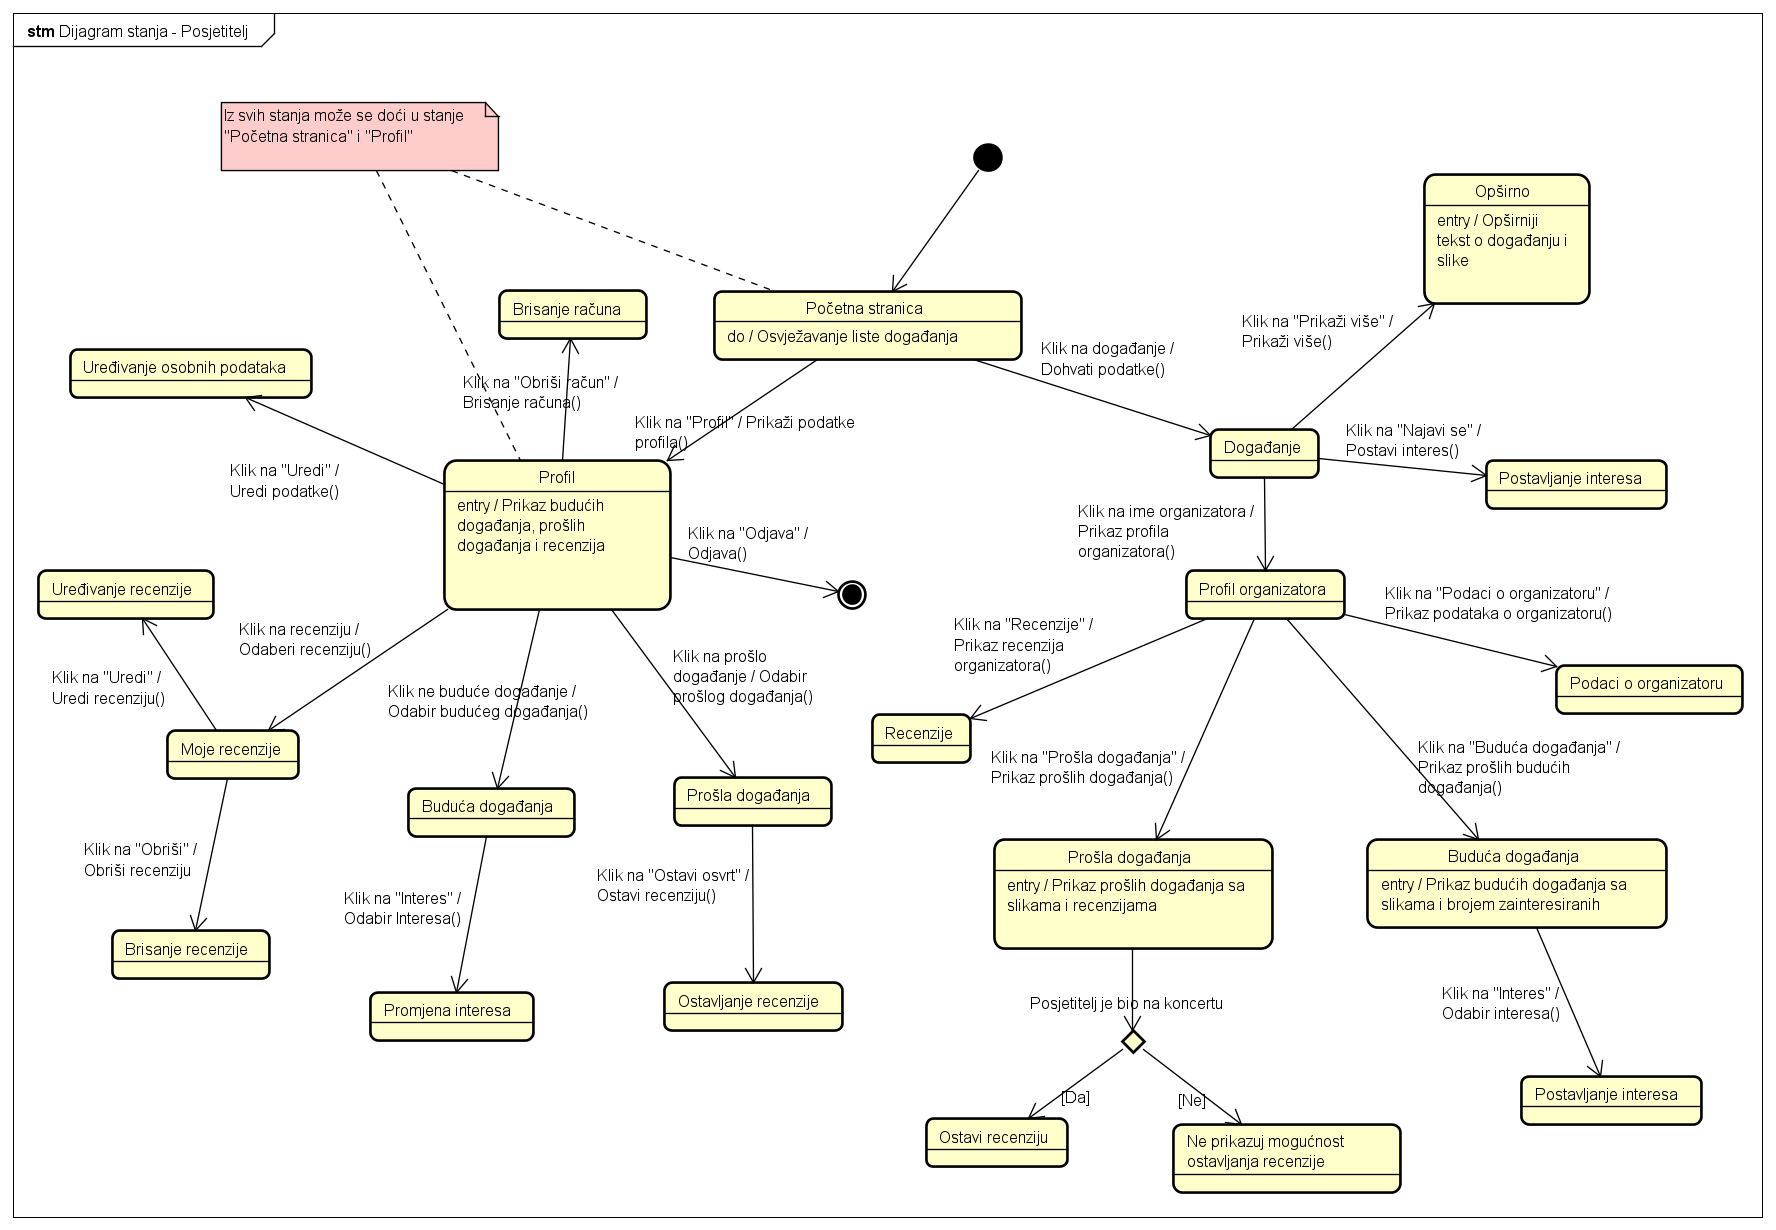
\includegraphics[width=\textwidth]{slike/Dijagram stanja - Posjetitelj.PNG} %veličina u odnosu na širinu linije
			\caption{Dijagram stanja - Posjetitelj}
			\label{fig:DSP} %label mora biti drugaciji za svaku sliku
		\end{figure}
			
			
			\eject 
		
		\section{Dijagram aktivnosti}
		
			Dijagram aktivnosti primjenjuje se za opis modela toka upravljanja ili toka podataka. Kao i kod sekvencijskog dijagrama kod dijagrama aktivnosti poseban naglasak ima redosljed kojim se aktivnosti isvršavaju. Zbog manjka kompleksnosti sustava u nastavku se nalaze dva dijagama aktivnosti. Prvi dijagram (\ref{fig:DAPZ}) prikazuje operacije sustava potrebne za postavljanje interesa na određeni događaj koji se još nije dogodio. Drugi dijagram (\ref{fig:DAOR}) prikazuje što se sve mora dogoditi da bi posjetitelj uspješno ostavio recenziju na događaj koji se već dogodio. 
			
			\begin{figure}[H]
			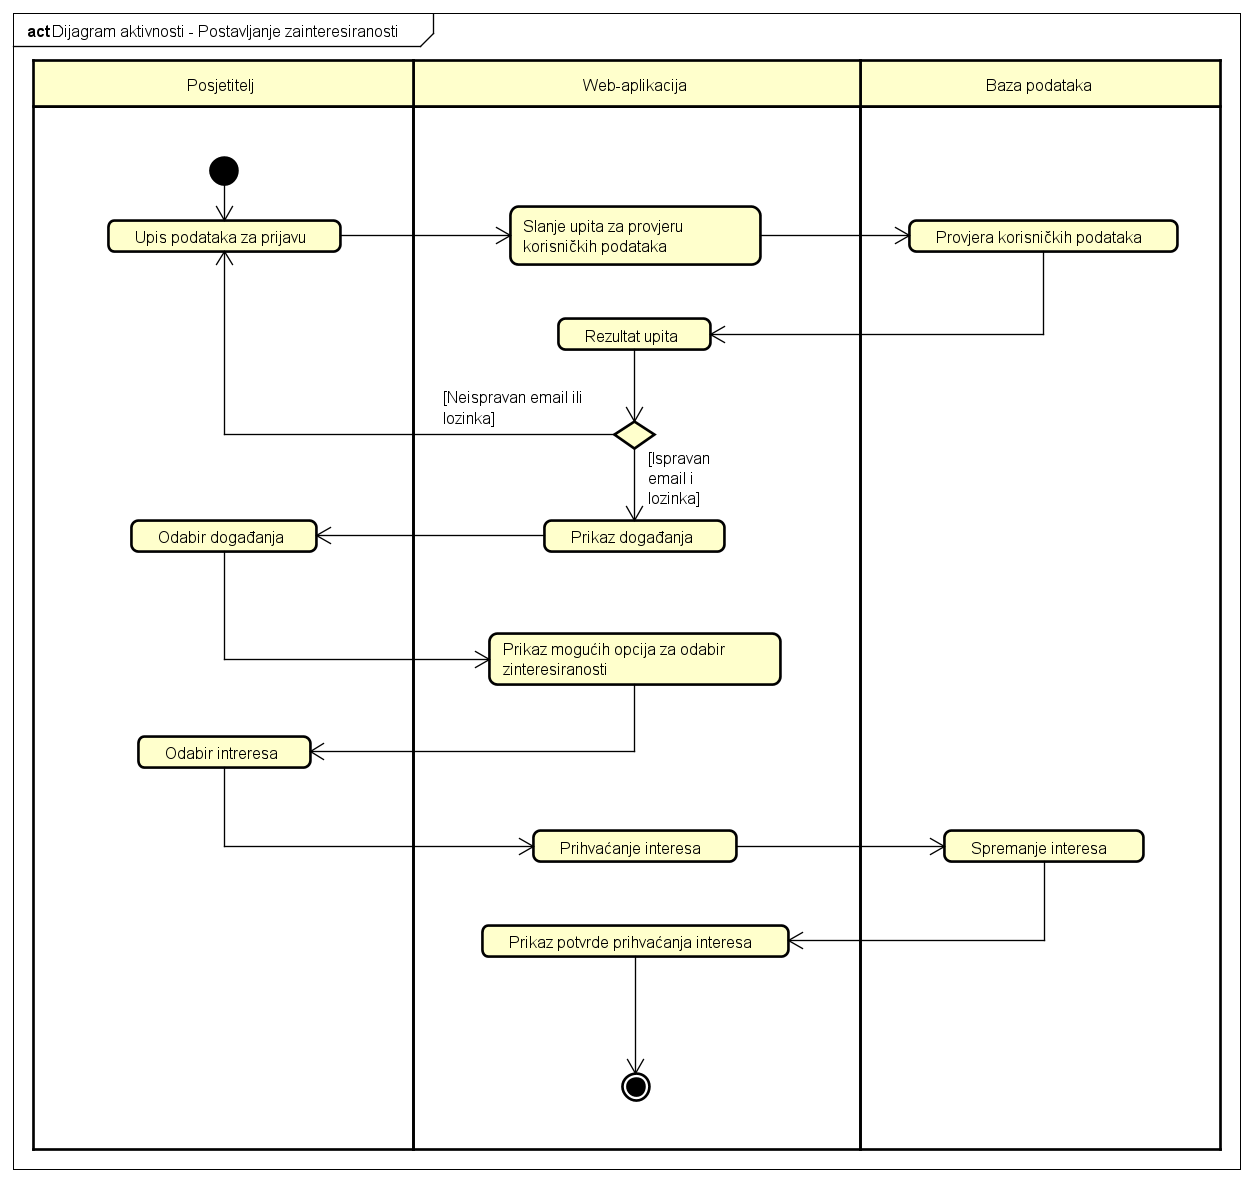
\includegraphics[width=\textwidth]{slike/Dijagram Aktivnosti - PZ.PNG} %veličina u odnosu na širinu linije
			\caption{Dijagram aktivnosti - Postavljanje zainteresiranosti}
			\label{fig:DAPZ} %label mora biti drugaciji za svaku sliku
		\end{figure}	
		
		\begin{figure}[H]
			\includegraphics[width=\textwidth]{slike/Dijagram Aktivnosti - OR.PNG} %veličina u odnosu na širinu linije
			\caption{Dijagram aktivnosti - Ostavljanje recenzije}
			\label{fig:DAOR} %label mora biti drugaciji za svaku sliku
		\end{figure}			
			
			\eject
		\section{Dijagram komponenti}
		
		Slika (\ref{fig:DK}) prikazuje dijagram komponenti. Dijagram opisuje unutranju strukturu sustava. Kako bi aplikacija funkcionirala frontend dio aplikacije se povezuje dvama sučeljima sa samom aplikacijom. Prvo mu sučelje služi za dohvaćanje HTML, JS i CSS datoteka. Aplikacije koristi Browser router za preusmjeravanje datoteka koje se trebaju poslati na sučelje. JavaScript datoteke koje Browser router može poslužiti nazvane su po prikazima(\textit{View}) koji se mogu otvoriti u poslužitelju. Iste te datoteke koriste React o kojem ovise u izgradnji izgleda svih komponenata stranice. S druge strane za dohvat JSON podataka koristi se sučelje koje je povezano s REST API komponentom. REST API služi za posluživanje podataka koji pripadaju backend djelu. Repository dohvaća dokumente iz same MongoDB baze i preko MVC arhitekture ih šalje na obradu. Unutar frontend aplikacije nalazi se komponenta Reactview koja pomoću sučelja izmjenjuje podatke s aplikacijom i otvara ili osvježava prikaze u poslužitelju.
						 
			 \begin{figure}[H]
			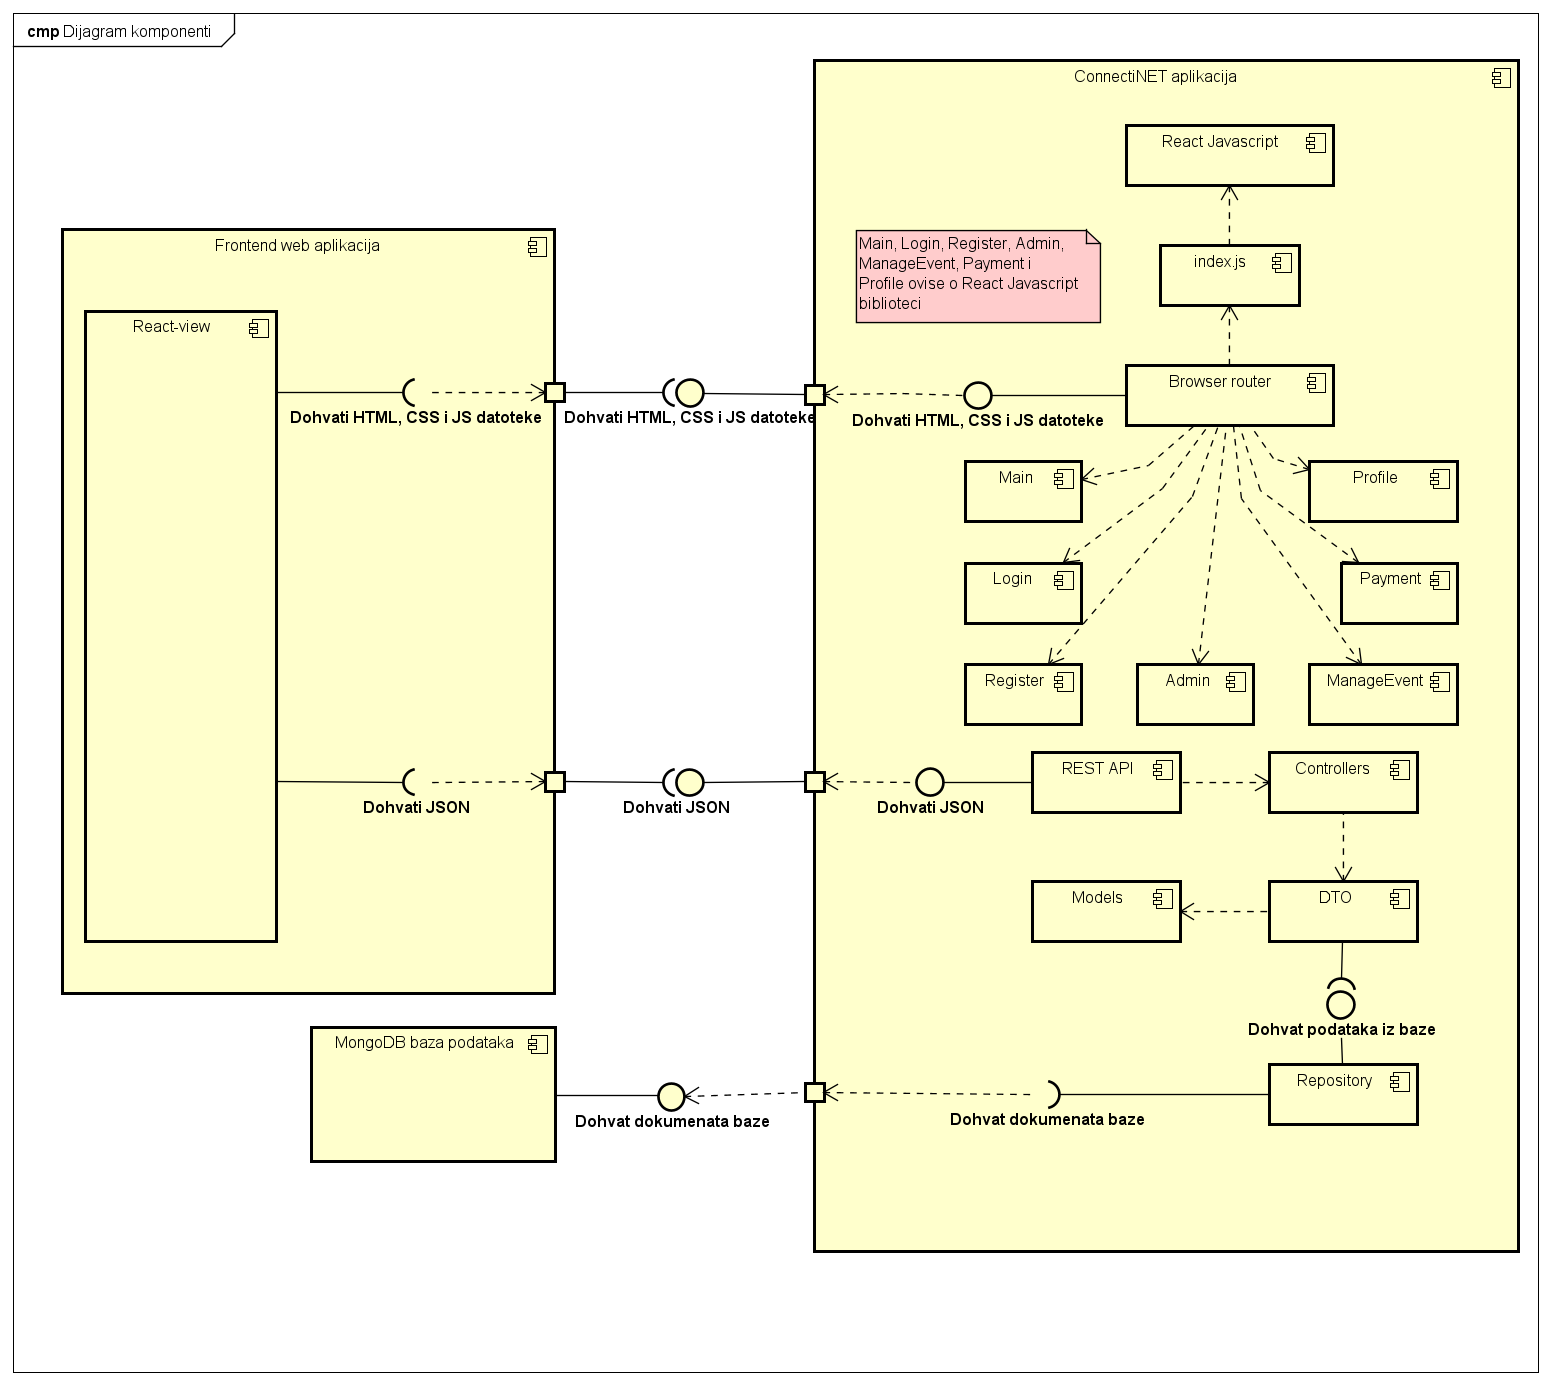
\includegraphics[width=\textwidth]{slike/Dijagram komponenti.PNG} %veličina u odnosu na širinu linije
			\caption{Dijagram komponenti}
			\label{fig:DK} %label mora biti drugaciji za svaku sliku
		\end{figure}